\newpage
\section*{Capítulo 2. Contexto y caracterización del caso de estudio}
\addcontentsline{toc}{section}{Capítulo 2. Contexto y caracterización del caso de estudio}
\setcounter{section}{2}
\setcounter{subsection}{0}

En este capítulo se presenta el contexto y la caracterización del caso de estudio, describiendo las condiciones del bosque seleccionado, las especies hospederas relevantes y su relación con la plaga de interés. Del mismo modo, se exponen los criterios técnicos que justifican su elección como escenario para la recolección de datos del proyecto.

\subsection{Justificación de la selección del área de interés}
La determinación del Bosque de Chapultepec como caso de estudio responde a la necesidad de encontrar un equilibrio entre la viabilidad logística, la relevancia biológica del problema y la pertinencia para la detección temprana. A diferencia de otras zonas forestales urbanas de la Ciudad de México —como el Bosque de San Juan de Aragón, con aproximadamente 2,500 árboles infestados y el 60\% en tratamiento activo, o Milpa Alta, con más de 2,100 árboles muertos documentados—, Chapultepec representa un escenario donde la plaga está presente pero aún no ha alcanzado niveles críticos de colapso \cite{mora2022chapultepec}. Esto lo convierte en el entorno idóneo para el desarrollo y validación de un sistema orientado a la \textbf{detección temprana}, que es precisamente donde la intervención tecnológica tiene mayor impacto. Los criterios considerados son los siguientes:

\begin{itemize}
    \item \textbf{Incidencia de la plaga:} El sitio presenta niveles de infestación documentados y focalizados por especie. Se reportan incidencias del 2.4\% en la población de fresnos (\textit{Hylesinus sp.}) y del 4.08\% en cedros (\textit{Phloeosinus sp.}) \cite{resendiz2019salud}. Estos porcentajes no reflejan la proporción del arbolado total del bosque, sino la fracción afectada 
    dentro de cada especie en particular. Para dimensionar su relevancia, cabe señalar que el promedio de afectación por descortezadores en el conjunto del arbolado urbano de la Ciudad de México alcanza el 30\% \cite{vega2022mongabay}; en este contexto, Chapultepec representa un foco activo pero con margen real de intervención preventiva.

    \item \textbf{Diversidad de muestras para el dataset:} La densidad de hospederos en el área, combinada con la variabilidad en el grado de avance de la infestación —desde individuos sanos hasta árboles con síntomas visibles en distintas etapas—, permite capturar imágenes representativas de múltiples estadios del daño. Esta diversidad es fundamental para construir un conjunto de datos con capacidad de generalización durante el entrenamiento del modelo de 
    clasificación \cite{resendiz2019salud}.

    \item \textbf{Accesibilidad y logística:} Las secciones II y III del bosque permanecen abiertas las 24 horas, mientras que la primera sección opera de martes a domingo en horario extendido. Esta flexibilidad facilita visitas recurrentes para la recolección de datos bajo distintas condiciones de iluminación natural, aspecto crítico para la robustez del sistema de visión por computadora.

    \item \textbf{Impacto ecológico y social:} Los bosques urbanos de esta escala contribuyen directamente a la calidad de vida de la población al mejorar la calidad del aire, regular la temperatura local y ofrecer servicios ecosistémicos esenciales \cite{forestal2025bosques}. La pérdida acelerada del arbolado en este sitio tendría consecuencias directas sobre millones de habitantes y visitantes, lo que refuerza la pertinencia de desarrollar herramientas tecnológicas de apoyo a su gestión sanitaria.
\end{itemize}

\subsection{Descripción General del Área de Estudio}
El Bosque de Chapultepec es el área verde urbana de mayor extensión y relevancia en la Ciudad de México. Su importancia trasciende lo ambiental, constituyendo un referente del patrimonio histórico, cultural y recreativo del país 
\cite{mora2022chapultepec}.

\begin{itemize}
    \item \textbf{Localización y extensión:} Se sitúa en las alcaldías Miguel Hidalgo (Secciones I, II y III) y Álvaro Obregón (Sección IV), abarcando una superficie total aproximada de 866.37 hectáreas, lo que lo posiciona como uno de los pulmones verdes más grandes de América Latina.

    \item \textbf{Valor social:} El área alberga museos, centros deportivos, lagos y monumentos de relevancia nacional, recibiendo a miles de visitantes diariamente \cite{mora2022chapultepec}. Este contexto subraya la urgencia de mantener la salud del arbolado, cuyo deterioro no solo implica pérdida ecológica sino también afectación directa al uso público del espacio.
\end{itemize}

\subsection{Caracterización de los Huespedes}

Dentro de los principales agentes bióticos que amenazan la salud de los bosques templados se encuentran los insectos descortezadores, un grupo de coleópteros de la familia \textit{Curculionidae} cuya característica distintiva es su vida subcortical: todo su ciclo reproductivo y alimenticio transcurre por debajo de la corteza de los árboles que colonizan \cite{delval_saenzromero2017descortezadores}. A pesar de su reducido tamaño (entre 0.1 y 0.6 cm) su capacidad de daño es considerable, ya que al establecerse en el interior del árbol comprometen directamente los tejidos responsables del transporte de nutrientes.

Aunque en el mundo se han descrito cerca de 3{,}000 especies de este grupo y en México están presentes 870 de ellas distribuidas en 87 géneros \cite{delval_saenzromero2017descortezadores}, no todas representan una amenaza equivalente para el arbolado. La gran mayoría mantiene poblaciones reducidas y cumple un papel regulador dentro del ecosistema forestal, eliminando individuos enfermos o debilitados y favoreciendo la renovación del dosel. Las especies con capacidad real de provocar la muerte del árbol por sí mismas son menos de 20 en el país, y pertenecen principalmente a los géneros \textit{Dendroctonus} e \textit{Ips} \cite{delval_saenzromero2017descortezadores}.

\begin{figure}[H]
    \centering
     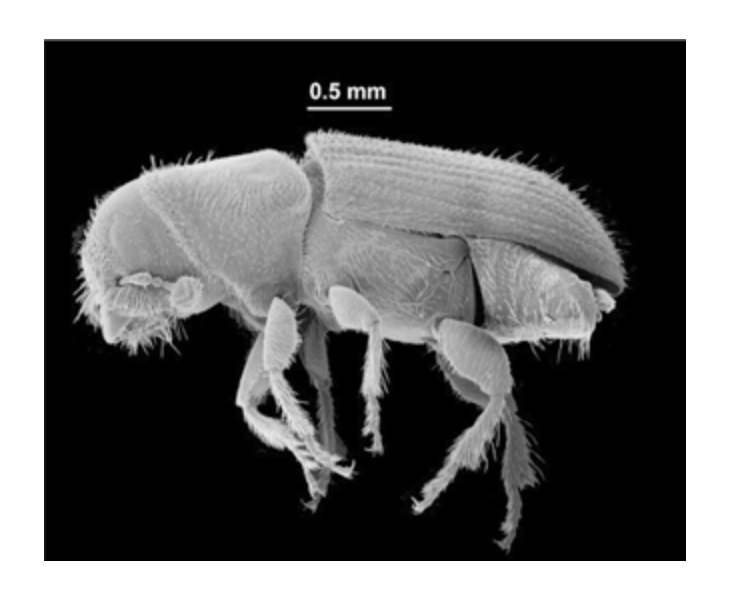
\includegraphics[width=0.55\textwidth]{images/C2/scabarajo.png}
    \caption{Escarabajo descortezador del pino \textit{Dendroctonus frontalis}. Tomado de \cite{delval_saenzromero2017descortezadores}}
    \label{fig:dendroctonus_frontalis}
\end{figure}

\subsubsection{Mecanismo de colonización y daño}

El proceso de colonización comienza con la perforación de la corteza por parte de la hembra adulta, que busca establecerse en el floema para alimentarse. La presencia de la hembra atrae al macho mediante señales químicas, y ambos inician la reproducción dentro del árbol. La hembra deposita sus huevos a lo largo de una galería central, cuidando que queden suficientemente separados para que las larvas no interfieran entre sí al alimentarse. Conforme cada larva se desarrolla, excava su propio recorrido subcortical, generando una red ramificada de galerías que se extiende desde el punto de entrada original. Este proceso de excavación y alimentación progresiva interrumpe los tejidos conductores de nutrientes del árbol de forma creciente hasta comprometer su viabilidad \cite{delval_saenzromero2017descortezadores}.

Un aspecto relevante para el presente proyecto es que cada especie de descortezador genera un patrón de galerías propio en la madera del hospedero \cite{delval_saenzromero2017descortezadores}. Si bien el sistema desarrollado no busca identificar la especie causante ni el árbol afectado de forma individual, la presencia de estos patrones subcorticales constituye en términos generales una evidencia visual directa de infestación activa. Es precisamente esta asociación entre la existencia de galerías y la clase "con infestación" la que el modelo de clasificación busca aprender a reconocer a partir de las imágenes del dataset.

\begin{figure}[H]
    \centering 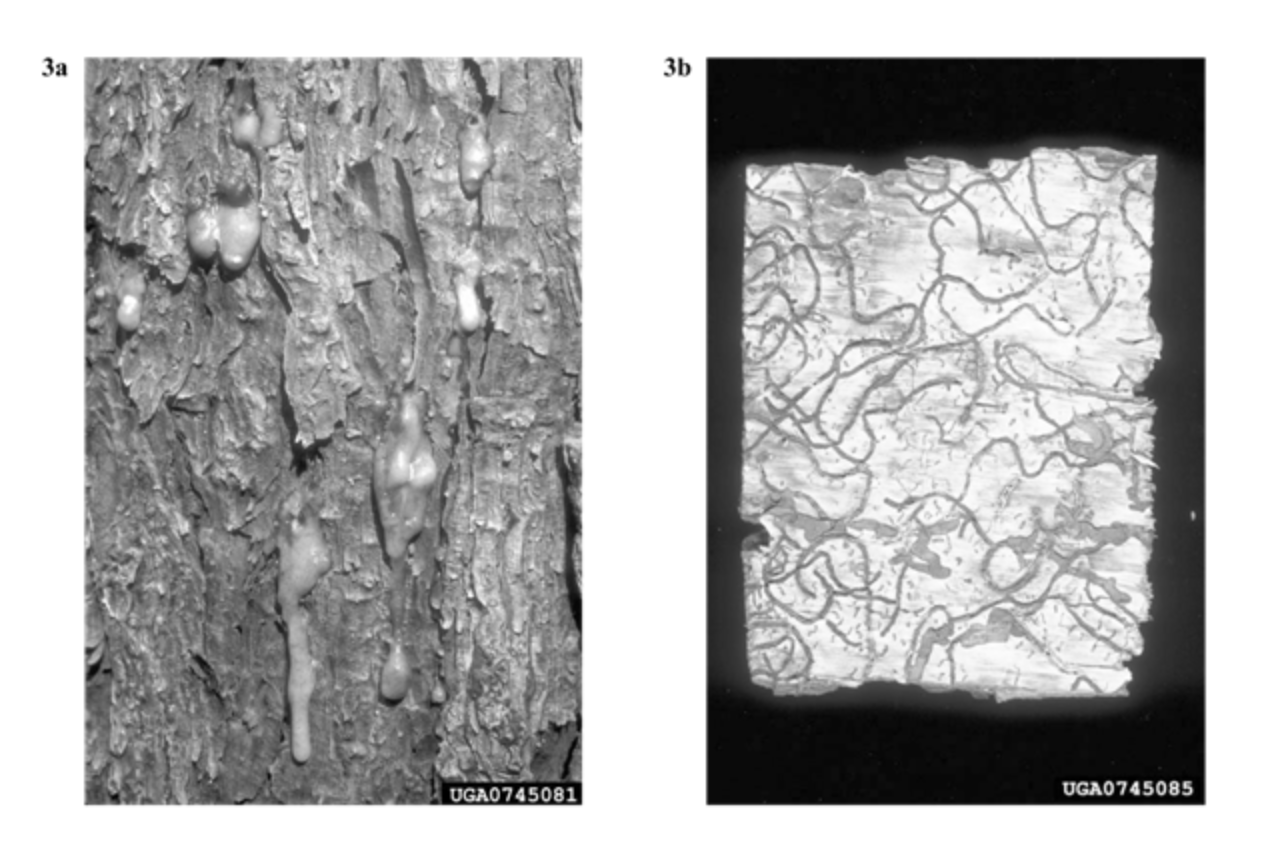
\includegraphics[width=0.7\textwidth]{images/C2/ABEFIGURE.png}
    \caption{a) Tronco de árbol con grumos de resina producidos como respuesta defensiva ante la perforación por descortezadores; b) Red de galerías formadas por \textit{D. frontalis} en el tejido subcortical. Tomado de \cite{delval_saenzromero2017descortezadores}}
    \label{fig:resina_galerias}
\end{figure}

\subsubsection{El papel de la resina como barrera de defensa}

Ante el ataque de los descortezadores, el árbol activa su principal mecanismo de defensa: la producción de resina, una sustancia viscosa almacenada bajo presión en conductos especializados del xilema. Cuando un insecto perfora la corteza, el árbol libera un flujo de resina que puede expulsar físicamente al atacante y sellar el orificio de entrada al endurecerse en contacto con el aire. Un árbol en condiciones fisiológicas óptimas puede sostener esta respuesta de forma efectiva. Sin embargo, cuando el árbol se encuentra debilitado por factores como la sequía, la edad o el estrés ambiental, la producción de resina disminuye o cesa, dejando al árbol sin su principal línea de defensa y permitiendo que los insectos accedan al floema sin resistencia, lo que a menudo conduce a su muerte \cite{delval_saenzromero2017descortezadores}.

\subsection{Caracterización de los Hospederos}
Para el desarrollo del sistema, es relevante identificar las especies que presentan mayor susceptibilidad ante los insectos descortezadores en el área de estudio, ya que estas constituyen el objetivo primario de detección y conforman una muestra significativa del dataset de entrenamiento. Si bien el sistema está diseñado para generalizar a otras especies arbóreas, los hospederos con mayor incidencia documentada representan los casos de referencia sobre los que se construye y valida el modelo.

\begin{itemize}
    \item \textbf{Fresnos (\textit{Fraxinus uhdei}):} Es la especie con mayor incidencia documentada de afecciones en el bosque. Su infestación por \textit{Hylesinus sp.} genera patrones de daño visibles en la corteza que constituyen el principal objetivo de detección mediante visión por computadora 
    \cite{resendiz2019salud}.

    \item \textbf{Cedros Blancos (\textit{Cupressus lusitanica}):} Presentan infestaciones vinculadas al estrés hídrico, que favorece la colonización por \textit{Phloeosinus sp.} Los individuos afectados manifiestan alteraciones visuales características en la textura y coloración de la corteza, señales que el sistema busca aprender a identificar de forma automatizada \cite{resendiz2019salud}.
\end{itemize}


\subsubsection{Condiciones de vulnerabilidad y contexto urbano}

La relación entre el debilitamiento fisiológico del arbolado y la susceptibilidad al ataque por descortezadores adquiere especial relevancia en entornos urbanos como el Bosque de Chapultepec. El estrés hídrico al que están sometidos los árboles en ecosistemas urbanos, agravado por las condiciones de impermeabilización del suelo, la contaminación y los efectos del cambio climático, reproduce el mismo patrón de vulnerabilidad documentado en bosques templados bajo condiciones de sequía \cite{delval_saenzromero2017descortezadores}.

\begin{figure}[H]
    \centering
     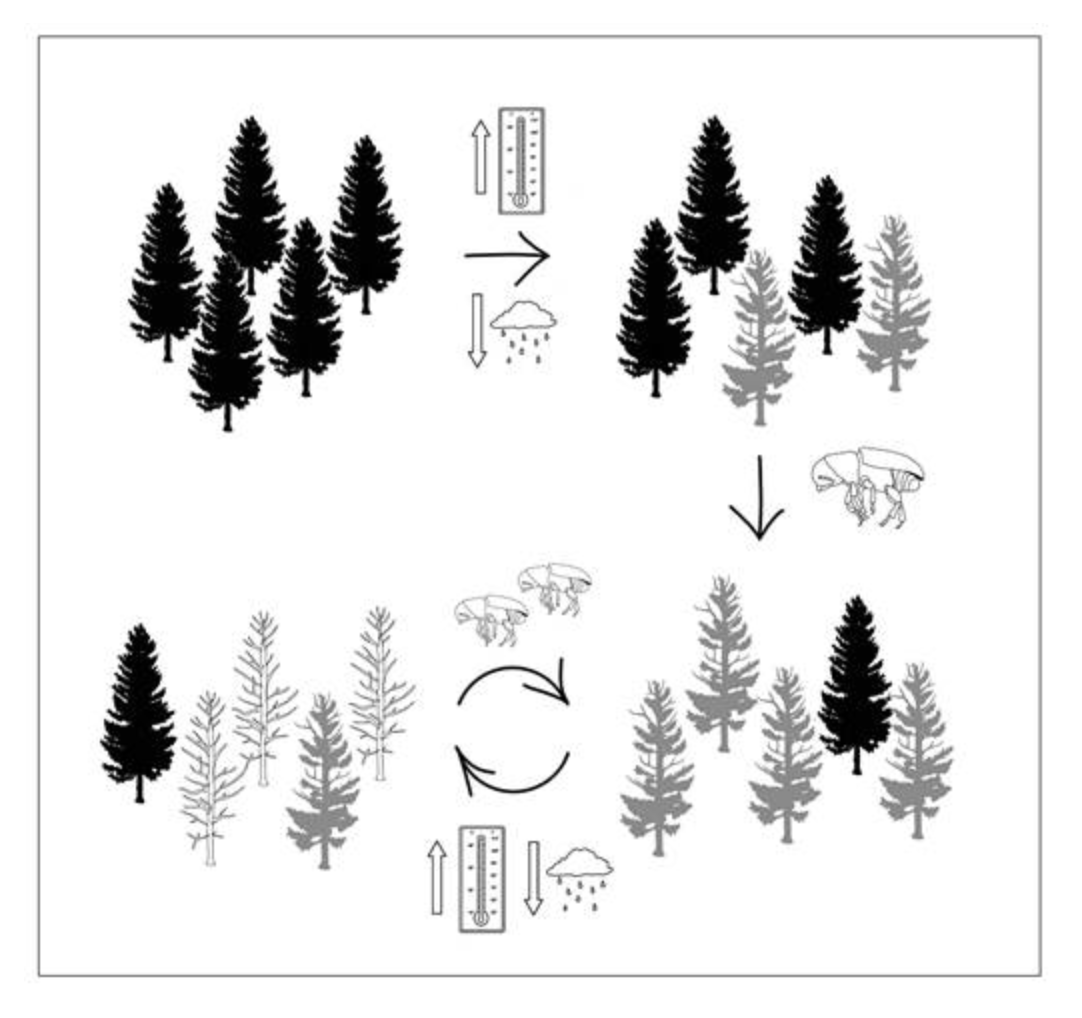
\includegraphics[width=0.6\textwidth]{images/C2/cicloRetro.png}
    \caption{Ciclo de retroalimentación negativa entre el cambio climático, el debilitamiento del arbolado y el incremento en la actividad de insectos descortezadores. Tomado de \cite{delval_saenzromero2017descortezadores}}
    \label{fig:ciclo_descortezadores}
\end{figure}

Este ciclo explica por qué las infestaciones por \textit{Hylesinus} sp.\ en \textit{Fraxinus uhdei} y por \textit{Phloeosinus} sp.\ en \textit{Cupressus lusitanica} documentadas en el área de estudio no son fenómenos aislados, sino manifestaciones locales de una dinámica forestal más amplia \cite{delval_saenzromero2017descortezadores}.
 Su detección oportuna tiene además una dimensión preventiva, ya que al identificar tempranamente la presencia de estos \textbf{descortezadores secundarios}, se posibilita la intervención antes de que el deterioro del arbolado genere condiciones propicias para la colonización por géneros de alto impacto como \textit{Dendroctonus e Ips}, cuya presencia implicaría un escenario de difícil o imposible reversión. En este sentido, el sistema no se limita a detectar infestaciones activas, sino que actúa como barrera preventiva frente a plagas de mayor severidad. 
 
 Comprender la biología de estos insectos y el proceso mediante el cual dañan al árbol es, por tanto, el punto de partida necesario para definir las señales visuales de interés que el sistema de clasificación busca aprender a identificar, descritas en detalle en las secciones siguientes.

\subsection{Progresión visual de la infestación por insectos descortezadores}

La detección visual de infestaciones por descortezadores puede abordarse desde dos niveles de observación complementarios, cada uno con señales cromáticas y morfológicas propias: el follaje, observable desde captura aérea, y la corteza, analizable a escala de árbol individual. Esta distinción es fundamental para el presente proyecto, ya que ambos niveles corresponden directamente a las imágenes que conforman el \textit{dataset} de entrenamiento descritos en la Sección 2.4.

\subsubsection{Señales visuales en el follaje}

Las alteraciones en el follaje constituyen la señal observable a escala macro, y son las que se capturan mediante dron en el primer nivel de análisis del sistema. De acuerdo con Gómez-Pineda y Ramírez \cite{gomez_pineda_ramirez2023descortezadores}, la progresión documentada en campo sigue la siguiente secuencia cromática. 

\begin{itemize}
    \item \textbf{Fase 1 --- Colonización reciente.} La coloración del follaje aún es \textbf{verde}, sin alteraciones cromáticas visibles desde el dosel. Sin embargo, a nivel de tronco ya se observan grumos frescos de resina blanca o rojiza sobre la corteza o ramas, así como desechos tipo aserrín en la base del árbol, señales de que la colonización subcortical ya ha comenzado.

    \item \textbf{Fase 2 --- Deterioro activo.} Conforme los descortezadores se reproducen y alimentan dentro del árbol, el follaje transita de verde a \textbf{verde-amarillento o verde limón}. En esta fase la infestación ya está activa y consolidada.

    \item \textbf{Fase 3 --- Muerte del árbol.} El follaje adquiere una coloración \textbf{roja o café-rojiza} generalizada. A lo largo del tronco se hace visible una gran cantidad de orificios de salida por donde emergieron las nuevas generaciones de insectos. El árbol ya está muerto y la corteza comienza a desprenderse con facilidad \cite{gomez_pineda_ramirez2023descortezadores}.
\end{itemize}

\begin{figure}[H]
    \centering
    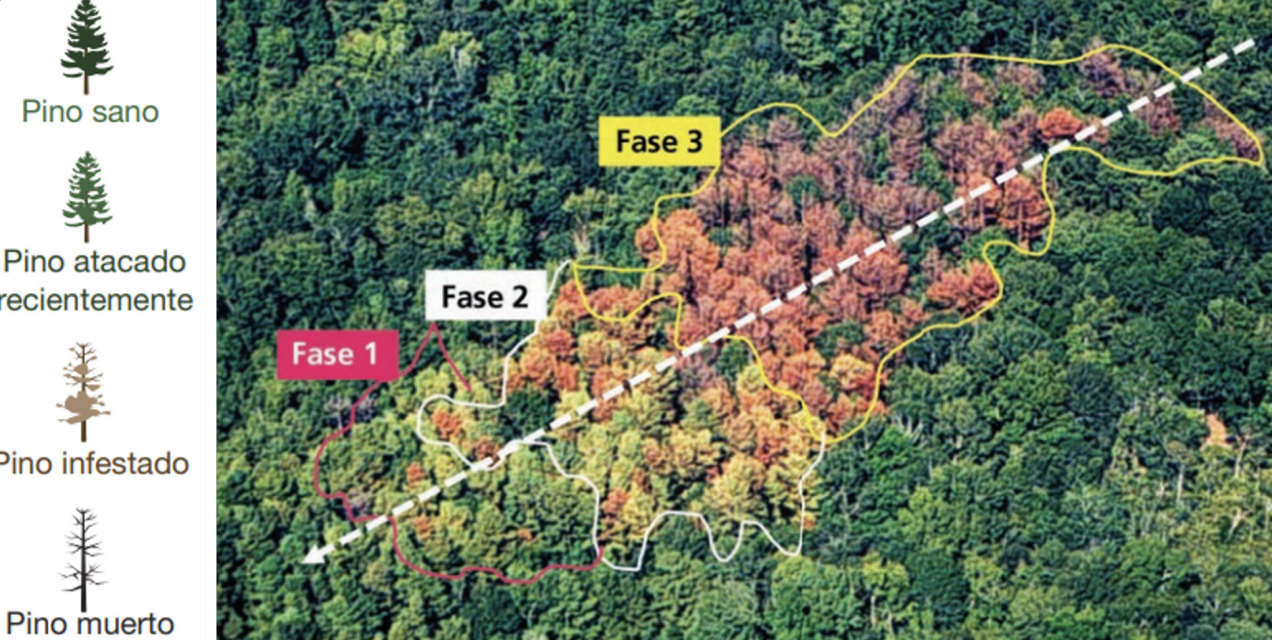
\includegraphics[width=1\textwidth]{images/C2/follaje.png}
    \caption{Etapas de coloración del follaje que indican la fase de infestación del arbolado. Se observa la transición de verde (Fase 1) a verde-amarillento (Fase 2) y café-rojizo (Fase 3), con la dirección de expansión del brote indicada. Tomado de \cite{gomez_pineda_ramirez2023descortezadores}}
    \label{fig:progresion_follaje}
\end{figure}

Un aspecto metodológicamente relevante de esta progresión es que durante la Fase 1 el follaje aún no presenta alteraciones cromáticas detectables desde el dosel, lo que limita la detección aérea temprana. Esto refuerza la necesidad del segundo nivel de análisis como mecanismo complementario de detección en estadios iniciales de infestación.

\subsubsection{Señales visuales en la corteza}

A escala de árbol individual, la infestación produce señales visibles tanto en la superficie exterior de la corteza como, de forma más directa, en el tejido subcortical expuesto mediante remoción controlada \cite{gomez_pineda_ramirez2023descortezadores}.

\textbf{En la superficie exterior de la corteza}

El proceso de colonización inicia cuando las hembras adultas perforan la corteza y se establecen en el floema. Como respuesta defensiva, el árbol produce resina que expulsa a los atacantes; sin embargo, cuando la infestación supera la capacidad de defensa del árbol, esta respuesta resulta insuficiente \cite{gomez_pineda_ramirez2023descortezadores}. Las señales visibles en la superficie exterior siguen la siguiente progresión:

\begin{itemize}
    \item \textbf{Fase 1 --- Respuesta defensiva activa.} Aparecen grumos frescos de resina en tonos \textbf{blancos, crema o rojizos} sobre el tronco y las ramas, junto con desechos tipo aserrín en la corteza y en la base del árbol. Estos son los primeros indicadores visibles de colonización activa, observables incluso cuando el follaje aún se mantiene verde.

    \item \textbf{Fase 2 --- Colonización avanzada.} Los exudados resinosos aumentan en volumen y comienzan a acumularse en tonos \textbf{café-anaranjados}. Simultáneamente aparecen pequeños orificios de entrada y salida de los insectos a lo largo del tronco, señal de que la población de descortezadores ya es numerosa.

    \item \textbf{Fase 3 --- Árbol muerto y abandonado.} La corteza presenta una coloración \textbf{café-grisácea uniforme}, sin exudados resinosos activos. Los orificios de emergencia son abundantes y evidentes. El árbol ha sido abandonado por los descortezadores primarios y comienza a ser colonizado por especies secundarias.
\end{itemize}

\textbf{En el tejido subcortical expuesto}

Mediante remoción controlada de la corteza externa, se exponen directamente las galerías excavadas por los insectos para alimentarse y ovipositar.  

\begin{figure}[H]
    \centering
    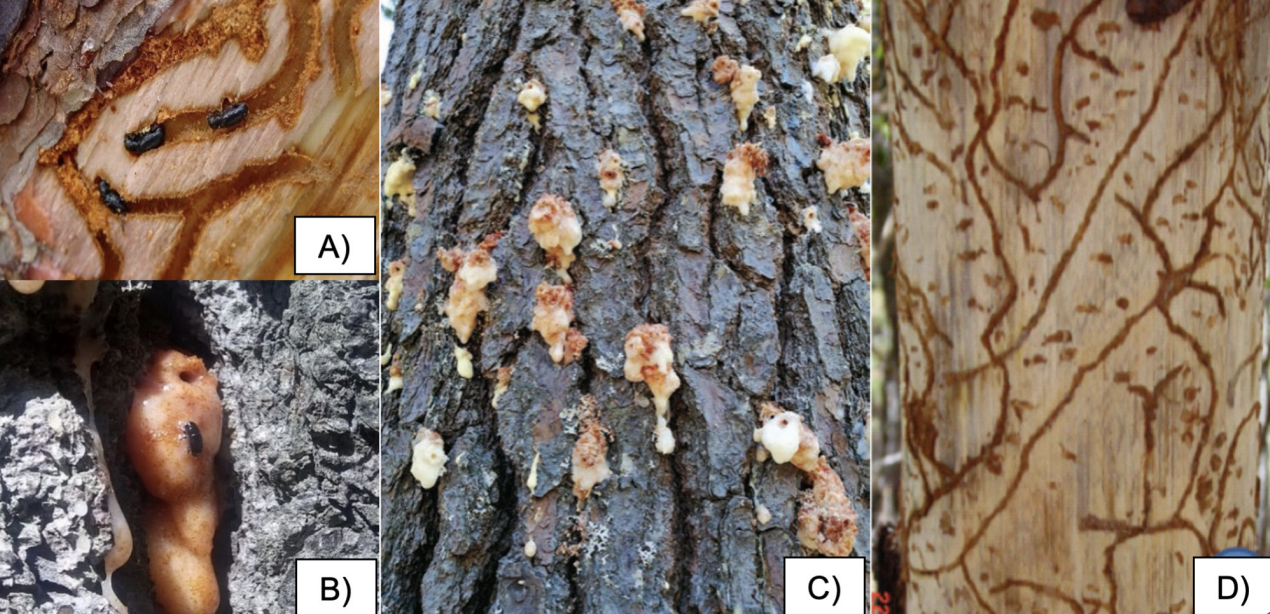
\includegraphics[width=0.8\textwidth]{images/C2/corteza.png}
    \caption{Señales visuales en la superficie exterior e interior de la corteza. A) hembras alimentándose en el tejido subcortical; B) macho entrando a través del orificio hecho por la hembra; C) grumos de resina acumulados a lo largo del tronco; D) galerías individuales generadas por las larvas durante la alimentación y oviposición. Tomado de \cite{gomez_pineda_ramirez2023descortezadores}}
    \label{fig:senales_corteza}
\end{figure}

La hembra excava una galería central mientras deposita huevos a cada lado; al eclosionar, las larvas generan galerías individuales ramificadas que se extienden interrumpiendo los tejidos conductores de nutrientes \cite{gomez_pineda_ramirez2023descortezadores}.

Estas estructuras presentan patrones cromáticos característicos: tonos \textbf{café-rojizos y anaranjados} en el tejido dañado, con trayectorias de excavación sobre un fondo de madera en tonos \textbf{beige y crema}. La presencia de estos patrones constituye la señal más directa y confiable de infestación activa, y representa la clase de mayor interés para el entrenamiento del modelo de clasificación.

\subsubsection{Implicaciones para el análisis de color del \textit{dataset}}

La diferenciación entre señales de follaje y señales de corteza tiene consecuencias metodológicas directas para el análisis cromático complementario propuesto en el Capítulo 6. Dado que cada tipo de imagen opera en un espacio visual distinto, el análisis de distribución cromática se plantea de forma \textbf{separada para cada nivel}, evitando generalizaciones que mezclen señales de naturaleza diferente.

Además, esta progresión muestra que las señales visibles en la corteza aparecen antes que los cambios en el follaje. Es decir, en una etapa temprana, la infestación ya puede observarse en la corteza mientras el árbol todavía conserva un aspecto verde en su copa.Esto es importante porque sugiere que las imágenes de corteza pueden ser más útiles para la detección temprana; sin embargo, también conviene considerar las imágenes del follaje, ya que constituyen un factor importante para complementar el análisis. Por tanto, esto representa un argumento adicional para incorporar ambos niveles de forma complementaria dentro del sistema.

Finalmente, aunque las referencias bibliográficas de base corresponden principalmente a coníferas del centro de México, las señales descritas son respuestas fisiológicas generales al daño en el floema, documentadas en múltiples géneros de árboles, por lo tanto, el presente proyecto las utiliza como \textbf{marco conceptual de referencia}.